\chapter{Fundamental concepts of ML}\label{ch-03}

Lectures 2 and 3 provide the \textbf{overview and terminology} of
Machine Learning before getting into actual models. We start from the
general picture --- learning as the approximation of an unknown
function from examples --- and then describe the ``ingredients'' of an
ML system (data, task, model, learning algorithm, validation) and three
crucial concepts: \textbf{inductive bias}, the \textbf{loss function}
and \textbf{generalisation}. Many concepts only hinted at here will be
taken up again and explored in the rest of the course.

\section{Machine Learning in the computational
setting}\label{il-machine-learning-in-ambito-computazionale}

Restricting ourselves to the computational framework, ML studies
\textbf{principles, methods and algorithms for learning and
prediction}: the system learns from experience (known data) to tackle a
computational task, building a \textbf{model} (or \textbf{hypothesis})
to be used for making predictions.

The most widespread specific framework, and the one adopted by the
course, is the following: \textbf{infer a model, i.e.\ a function, from
a set of examples, so that it is able to generalise}, that is, to give
accurate answers on new data.

\subsection{When to use ML}\label{quando-usare-il-ml}

ML should be used with \textbf{opportunity} (when it is really needed)
and \textbf{awareness} (of its requirements and limits). Predictive
models are useful when:

\begin{itemize}
\tightlist
\item
  there is no theory (or little knowledge) explaining the phenomenon;
\item
  data are \textbf{uncertain, noisy or incomplete}, and this hinders
  the formalisation of an exact solution.
\end{itemize}

In exchange, ML requires two things: a \textbf{source of experience}
for training (\emph{representative} data) and a certain
\textbf{tolerance on the precision} of the results, which will never be
guaranteed to be exact.

ML is complementary to traditional techniques (analytical models based
on prior knowledge, algorithms and imperative programming, classical
AI). It is particularly suitable when:

\begin{itemize}
\tightlist
\item
  \textbf{knowledge is too hard to formalise} by hand: humans recognise
  faces but cannot describe \emph{how} they do it; the same holds for
  speech recognition;
\item
  \textbf{human knowledge is not enough}: for example, predicting the
  binding strength of molecules to proteins;
\item
  \textbf{personalised behaviour} is needed: filtering emails or web
  pages according to user preferences, individualised human--machine
  interfaces.
\end{itemize}

The great challenges of ML are building \textbf{intelligent autonomous
systems} (robotics, human--robot interaction, search engines),
providing \textbf{powerful tools for data analysis} (the tools of the
\emph{data scientist}) and opening \textbf{new interdisciplinary
application areas}, in an era in which scientific progress is
increasingly \emph{data-driven}.

\section{Learning as function
approximation}\label{lapprendimento-come-approssimazione-di-funzioni}

The course adopts a specific but very widespread view: \textbf{learning
is the approximation of an unknown function from examples}. The
advantage is that different tasks (classification, regression,
\ldots) are treated in a uniform framework --- mathematically, that of
function spaces (Hilbert spaces) --- which allows a rigorous
formulation.

\subsection{The guiding example: digit
recognition}\label{lesempio-guida-riconoscimento-di-cifre}

Let us go back to the example of the first lecture. The input is a
collection of images of handwritten digits (\(8\times 8\) matrices of
values); the problem is to build a model that, given an image,
\textbf{predicts} the digit. This is a \textbf{classification problem}
with ten classes.

It is a typical ML success case: it is \textbf{hard to formalise
exactly} the solution (handwriting varies, there is noise and there are
ambiguous data), while it is \textbf{relatively easy to collect labelled
examples}.

\begin{boxdefinition}{Machine Learning (extended definition)}

ML studies and proposes methods for building (\textbf{inferring})
dependencies, functions or hypotheses from examples of observed data,
that: - \textbf{fit} the known examples; - are able to
\textbf{generalise}, with reasonable accuracy, to new data;

according to \textbf{verifiable} results, under statistical and
computational conditions and criteria, taking into account the
\textbf{expressiveness} and \textbf{algorithmic complexity} of the
models and learning algorithms.

\end{boxdefinition}

\subsection{\texorpdfstring{Examples of pairs
\(x \to f(x)\)}{Examples of pairs x \textbackslash to f(x)}}\label{esempi-di-coppie-x-to-fx}

In all the following cases we want to infer a general function from
known data, i.e.\ from a \textbf{training set} (TR) of pairs
\(\langle x, f(x)\rangle\):

{\def\LTcaptype{none} % do not increment counter
\begin{longtable}[]{@{}
  >{\raggedright\arraybackslash}p{(\linewidth - 4\tabcolsep) * \real{0.3333}}
  >{\raggedright\arraybackslash}p{(\linewidth - 4\tabcolsep) * \real{0.3333}}
  >{\raggedright\arraybackslash}p{(\linewidth - 4\tabcolsep) * \real{0.3333}}@{}}
\toprule\noalign{}
\begin{minipage}[b]{\linewidth}\raggedright
Problem
\end{minipage} & \begin{minipage}[b]{\linewidth}\raggedright
Input \(x\)
\end{minipage} & \begin{minipage}[b]{\linewidth}\raggedright
Output \(f(x)\)
\end{minipage} \\
\midrule\noalign{}
\endhead
\bottomrule\noalign{}
\endlastfoot
Handwriting recognition & pen movement data & letter of the
alphabet \\
Medical diagnosis & patient properties (symptoms, tests) & disease or
recommended therapy \\
Face recognition & bitmap of the face & name of the person \\
Spam detection & email message & spam / not spam \\
\emph{Protein folding} & amino acid sequence (variable-length string) &
3D coordinates of the atoms (sequence of vectors) \\
\emph{Drug design} & molecule (graph of atoms and bonds) & binding
strength to HIV protease (real number) \\
\end{longtable}
}

The last two examples show that inputs and outputs can be
\textbf{complex data}: strings, sequences, graphs.

\section{The ingredients of an ML
system}\label{gli-ingredienti-di-un-sistema-di-ml}

A predictive ML system can be described through its components, which
also constitute a \textbf{guide to the key design choices}.

\begin{figure}[htbp]
\centering
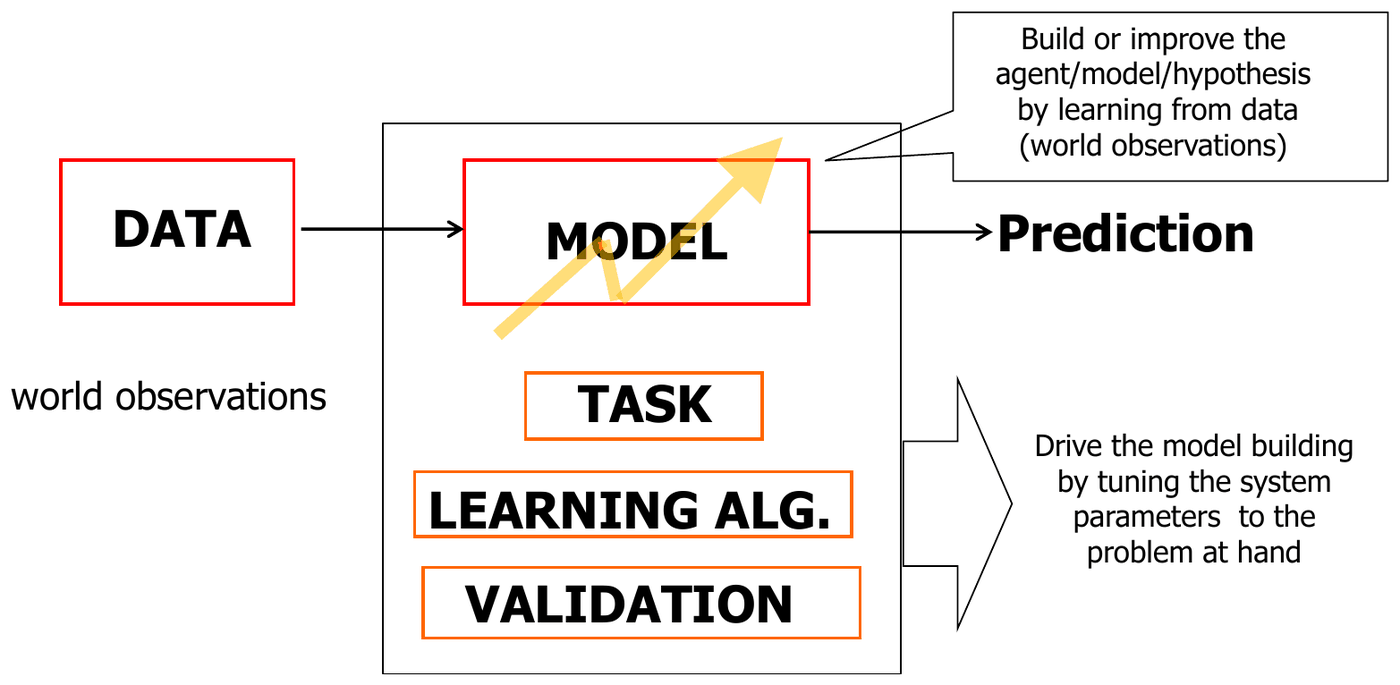
\includegraphics[width=0.86\linewidth,height=0.42\textheight,keepaspectratio]{images/03-l23_sistema-ml.png}
\caption{Overview of a predictive ML system and its ``ingredients''.}
\end{figure}

\begin{itemize}
\tightlist
\item
  \textbf{Data}: the observations of the world, i.e.\ the available
  experience.
\item
  \textbf{Task}: the purpose of the application, which defines what we
  want to obtain.
\item
  \textbf{Model}: the agent/hypothesis that is built or improved by
  learning from data.
\item
  \textbf{Learning algorithm}: drives the construction of the model by
  tuning the system's parameters to the problem.
\item
  \textbf{Validation}: evaluates the quality of the obtained model.
\end{itemize}

\subsection{Data}\label{dati}

Data represent the available facts. The first problem is that of
\textbf{representation}: how to capture the structure of the objects
being analysed.

In the \textbf{flat} case (attribute-value language) each object is a
\textbf{fixed-size vector of properties} (\emph{features}), and the
whole dataset is a table of tuples. Attributes can be
\textbf{categorical/discrete} (colour: yellow, red) or
\textbf{continuous} (weight, cost), and there may be \textbf{missing
data} (denoted by ``?'').

\begin{boxnote}{Data terminology}

\begin{itemize}
\tightlist
\item
  Each row \(\mathbf{x}\) (vector, in bold) is an \textbf{example},
  \emph{pattern}, instance, sample.
\item
  The \textbf{dataset size} is the number of examples, denoted by
  \(l\).
\item
  The \textbf{input dimension} is the number of features, denoted by
  \(n\).
\item
  \(x_i\) (or \(x_j\)) is typically the \(i\)-th feature (attribute,
  component) of \(\mathbf{x}\).
\item
  \(\mathbf{x}_p\) is typically the \(p\)-th pattern (row) of the
  dataset.
\item
  \(x_{p,i}\) is attribute \(i\) of pattern \(p\).
\end{itemize}

\end{boxnote}

Data can be \textbf{pre-processed}: variable scaling, encoding, feature
selection.

\subsubsection{Encoding categorical
variables}\label{codifica-delle-variabili-categoriche}

To use categorical variables in numerical models they must be encoded:

\begin{itemize}
\tightlist
\item
  for \textbf{two classes} one uses \(0/1\) or \(-1/+1\);
\item
  for \textbf{more classes} one can use \(1, 2, 3, \dots\), but this
  encoding introduces an artificial \textbf{degree of similarity}
  (class 1 turns out to be ``closer'' to 2 than to 3). It is suitable
  only for \textbf{ordered categorical} variables (e.g.\ small, medium,
  large);
\item
  for symbols without an order one uses the \textbf{1-of-k} (or
  \textbf{one-hot}) encoding: each symbol becomes a vector with a
  single 1, for example \(A = (1,0,0)\), \(B = (0,1,0)\),
  \(C = (0,0,1)\). All symbols are thus equidistant from each other. It
  is used for both input and output, and it is useful for the project.
\end{itemize}

\subsubsection{Structured data}\label{dati-strutturati}

Many data are not naturally vectors: \textbf{sequences} (lists),
\textbf{trees}, \textbf{graphs}, multi-relational data. Examples:
images, time series, strings of a language, DNA and proteins,
hierarchical relations, molecules, the link network of web pages. The
problem is finding a natural representation for them (this will be
discussed in the advanced part of the course).

\begin{figure}[htbp]
\centering
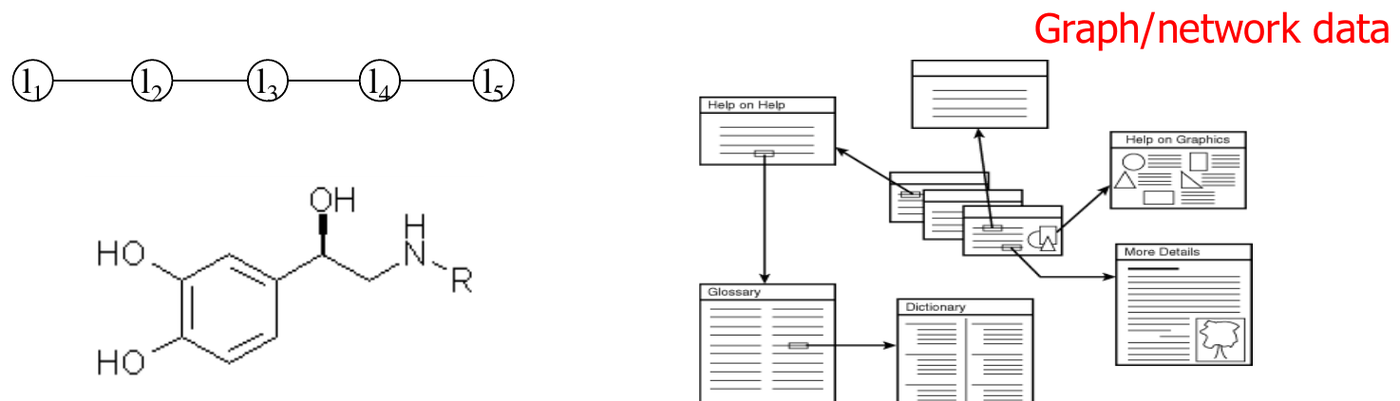
\includegraphics[width=0.74\linewidth,height=0.42\textheight,keepaspectratio]{images/03-l23_dati-strutturati.png}
\caption{Structured data: sequences, molecules and graphs.}
\end{figure}

\subsubsection{Noise, outliers and feature
selection}\label{rumore-outlier-e-feature-selection}

\begin{itemize}
\tightlist
\item
  \textbf{Noise} is the addition of external factors to the
  informative signal: it is due to the randomness of measurements, not
  to the underlying law (e.g.\ Gaussian noise).
\item
  \textbf{Outliers} are unusual values, inconsistent with most
  observations (e.g.\ anomalous measurement errors). They are handled
  by detecting and removing them in pre-processing or by using
  \textbf{robust} modelling methods.
\item
  \textbf{Feature selection} selects a small number of informative
  features, providing an optimal input representation for the problem.
\end{itemize}

\subsection{Task}\label{task}

The task defines the purpose of the application: what knowledge we
want to obtain, what the useful nature of the result is, what
information is available. We distinguish:

\begin{itemize}
\tightlist
\item
  \textbf{predictive tasks} (classification, regression): function
  approximation --- they are the focus of the course;
\item
  \textbf{descriptive tasks} (cluster analysis, association rules):
  finding subsets or groups of unclassified data.
\end{itemize}

\subsubsection{Supervised
learning}\label{apprendimento-supervisionato}

\begin{boxdefinition}{Supervised learning}

\textbf{Data}: training examples of the form
\(\langle \text{input}, \text{output}\rangle = \langle \mathbf{x}, d\rangle\)
(\textbf{labelled} examples) for an unknown function \(f\), known only
at the example points. The \textbf{target} \(d\) (also denoted by \(t\)
or \(y\)) is provided by a ``teacher'' according to \(f(\mathbf{x})\).

\textbf{Goal}: find a good approximation of \(f\), i.e.\ a
\textbf{hypothesis} \(h\) that can be used to predict on unseen data
\(\mathbf{x}'\) --- a hypothesis that \textbf{generalises}.

\end{boxdefinition}

The target can be:

\begin{itemize}
\tightlist
\item
  \textbf{categorical} → \textbf{classification}:
  \(f(\mathbf{x}) \in \{1, 2, \dots, K\}\) (discrete-valued function);
\item
  \textbf{numerical} → \textbf{regression}:
  \(f(\mathbf{x}) \in \mathbb{R}\) or \(\mathbb{R}^K\) (continuous
  real-valued function).
\end{itemize}

Thanks to the function approximation formalism, classification and
regression have a \textbf{unified view}. In statistical terminology,
inputs are the \textbf{independent variables} and outputs the
\textbf{dependent variables} or \textbf{responses}.

\subsubsection{Unsupervised
learning}\label{apprendimento-non-supervisionato}

In \textbf{unsupervised} learning there is no teacher: the training set
contains only \textbf{unlabelled} data \(\langle \mathbf{x}\rangle\).
The goal is for example to find \textbf{natural groupings} in the data
(\textbf{clustering}, i.e.\ partitioning the data into subsets of
``similar'' elements), to perform \textbf{dimensionality reduction},
visualisation or pre-processing, or to \textbf{model the density} of
the data.

\begin{figure}[htbp]
\centering
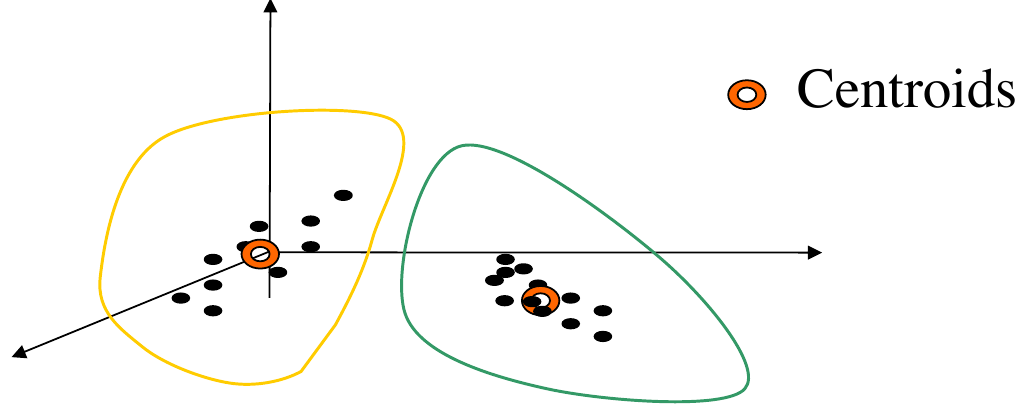
\includegraphics[width=0.60\linewidth,height=0.42\textheight,keepaspectratio]{images/03-l23_clustering.png}
\caption{Clustering: partition of the data into groups, each represented
by its centroid.}
\end{figure}

\subsubsection{Classification}\label{classificazione}

In classification, patterns are seen as members of a class, and the
goal is to assign each pattern to the correct class. If there are
\textbf{two} classes, \(f(\mathbf{x})\) is a \textbf{Boolean function}:
we speak of \textbf{binary classification} or \textbf{concept learning}
(true/false, \(0/1\), \(-1/+1\), negative/positive). With \textbf{more
than two} classes we have a \textbf{multi-class} problem.

Geometrically, classification can be seen as the \textbf{partition of
the input space into decision regions}. The simplest example is the
linear separator in \(\mathbb{R}^2\): a line (in general a hyperplane)
that separates the points of class 1 from those of class 0.

\begin{figure}[htbp]
\centering
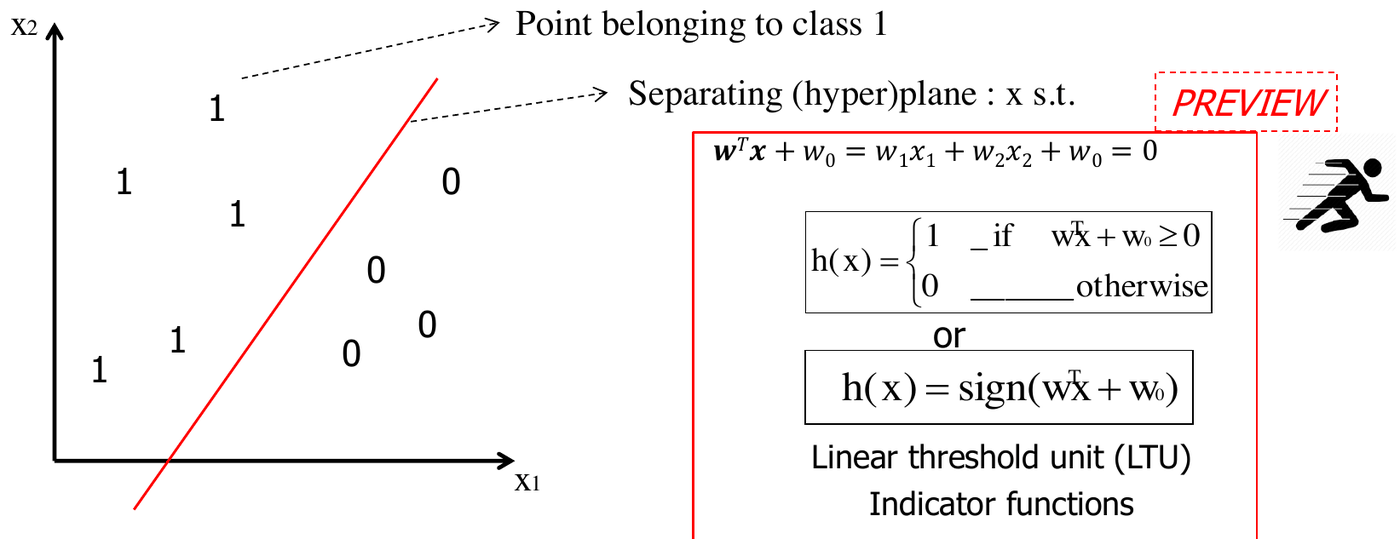
\includegraphics[width=0.89\linewidth,height=0.42\textheight,keepaspectratio]{images/03-l23_separatore-lineare.png}
\caption{A linear separator in the plane: a preview of the Linear
Threshold Unit.}
\end{figure}

The separating hyperplane is the set of points \(\mathbf{x}\) such that
\[
\mathbf{w}^T\mathbf{x} + w_0 = w_1 x_1 + w_2 x_2 + w_0 = 0,
\] and the classifier is \[
h(\mathbf{x}) = \begin{cases} 1 & \text{if } \mathbf{w}^T\mathbf{x} + w_0 \ge 0 \\ 0 & \text{otherwise} \end{cases}
\qquad \text{or} \qquad h(\mathbf{x}) = \operatorname{sign}(\mathbf{w}^T\mathbf{x} + w_0).
\] This model is called \textbf{Linear Threshold Unit} (LTU) and will
be studied in detail later. Functions of this kind, with values in
\(\{0,1\}\), are called \textbf{indicator functions}. The set \(H\) of
all dichotomies (splits into two classes) induced by hyperplanes is its
hypothesis space.

\begin{figure}[htbp]
\centering
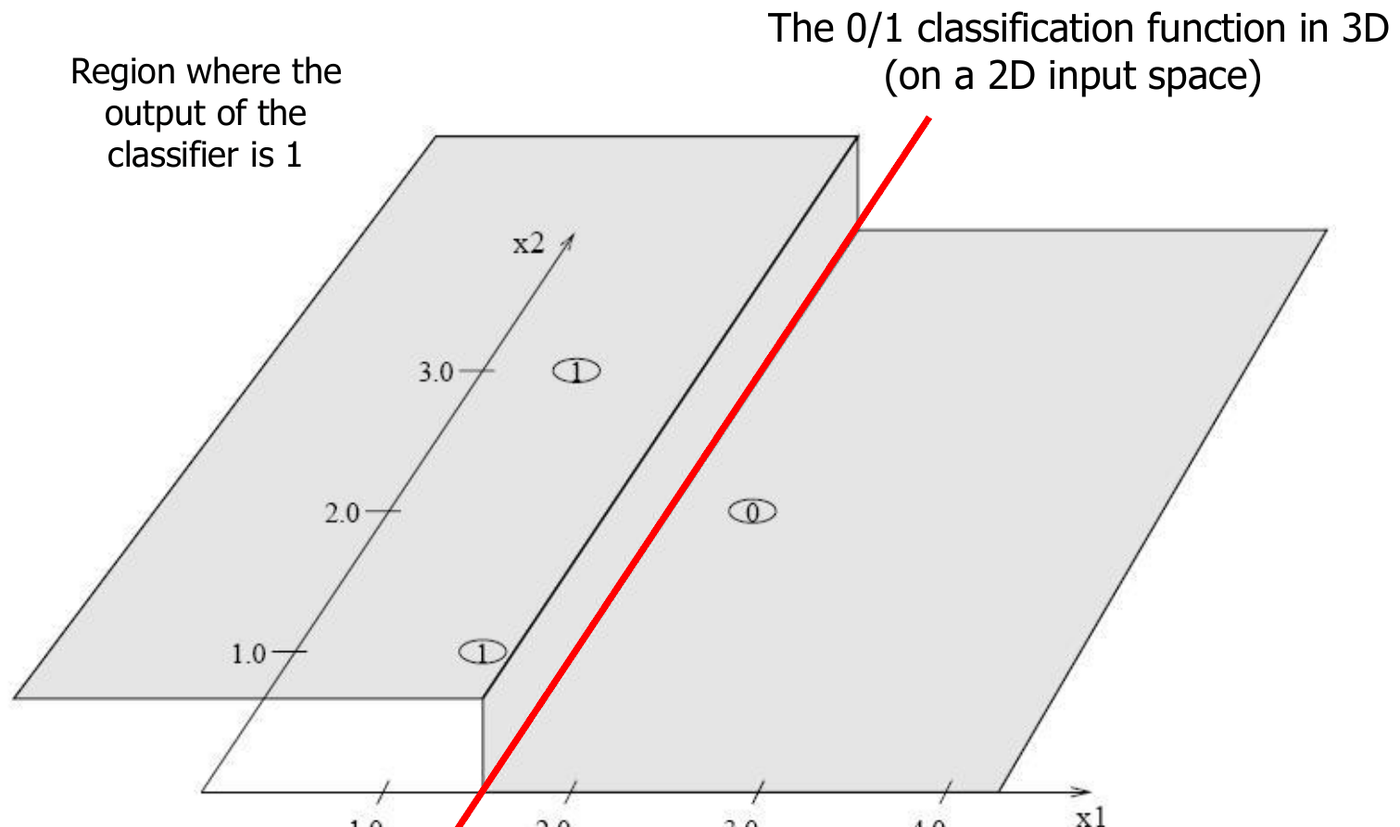
\includegraphics[width=0.77\linewidth,height=0.42\textheight,keepaspectratio]{images/03-l23_classificatore-3d.png}
\caption{The same classification function seen in 3D: it is a ``step''
function that is 1 in one region and 0 in the other.}
\end{figure}

\subsubsection{Regression}\label{regressione}

\textbf{Regression} is the estimation of a real-valued function on the
basis of a finite set of \textbf{noisy samples}: pairs
\((\mathbf{x}, f(\mathbf{x}) + \text{noise})\) are known. It is a form
of \emph{curve fitting} (in one dimension in the example, in \(k\)
dimensions in general).

\begin{boxexample}{Regression exercise}

Given the points \((1;\,2.1)\), \((2;\,3.9)\), \((3;\,6.1)\),
\((4;\,8.4)\), \((5;\,9.8)\), what is \(f\)? It comes naturally to
hypothesise \(f(x) = 2x\), which has small errors on all points. But
how did we choose it? And how would a machine (for example a neural
network) do it? This is exactly what the learning algorithm must
formalise.

\end{boxexample}

\begin{figure}[htbp]
\centering
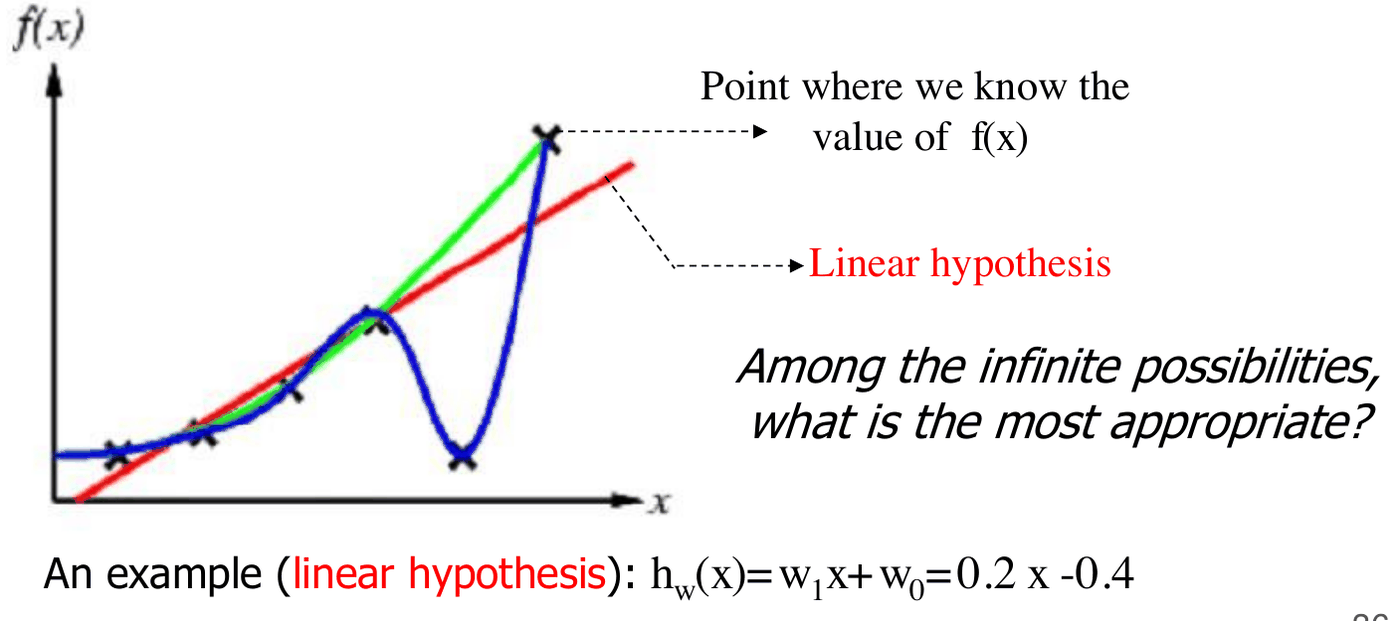
\includegraphics[width=0.77\linewidth,height=0.42\textheight,keepaspectratio]{images/03-l23_regressione.png}
\caption{Among the infinitely many functions compatible with the data,
which is the most appropriate?}
\end{figure}

The figure poses the key question: among infinitely many
possibilities, which function should we choose? The blue curve passes
exactly through all points but oscillates unnaturally; the red line
(\(h_\mathbf{w}(x) = w_1 x + w_0 = 0.2x - 0.4\)) makes small errors
but is much simpler. This dilemma is the heart of the problem of
\textbf{generalisation}.

\subsubsection{Other paradigms}\label{altri-paradigmi}

\begin{itemize}
\tightlist
\item
  \textbf{Semi-supervised learning}: combines labelled and unlabelled
  examples.
\item
  \textbf{Self-supervised learning}: a form of supervised learning in
  which the labels are \textbf{generated automatically from the
  structure of the data itself}, without manual labelling. The model is
  \textbf{pre-trained} on large amounts of unlabelled data, learning
  general representations, which are then adapted to specific tasks via
  \textbf{fine-tuning}. Current examples, at the basis of LLMs:

  \begin{itemize}
  \tightlist
  \item
    \textbf{next-word prediction} in a text, i.e.\ the
    \textbf{autoregressive} self-supervised learning of the GPT family
    (\emph{Generative Pre-trained Transformer}, OpenAI);
  \item
    reconstruction of \textbf{masked words} (BERT, Google);
  \item
    for images, \textbf{masked autoencoders} (Meta), which reconstruct
    hidden portions of the image.
  \end{itemize}
\item
  \textbf{Reinforcement learning}: learning with a ``critic'' that says
  right/wrong. The algorithm learns a \textbf{policy} on how to act
  given observations of the world; every action has an impact on the
  environment, which provides feedback. There are no step-by-step
  examples; the goal is \emph{decision-making}, and it is widely used
  in modern AI.
\end{itemize}

\subsection{Model}\label{modello}

The \textbf{model} captures the relationships among data (according to
the task) through a ``language'' (numerical, symbolic, \ldots), tied to
the representation used. Above all, \textbf{the model defines the class
of functions the machine can implement}: the \textbf{hypothesis space}.
For example, the set of functions \(h(\mathbf{x}, \mathbf{w})\) as the
parameter \(\mathbf{w}\) varies.

\begin{boxdefinition}{Basic terminology}

\begin{itemize}
\tightlist
\item
  \textbf{Training example} (supervised): pair
  \((\mathbf{x}, f(\mathbf{x}) + \text{noise})\), where \(\mathbf{x}\)
  is the feature vector and \(d = f(\mathbf{x}) + \text{noise}\) is the
  \textbf{target}.
\item
  \textbf{Target function} \(f\): the true (unknown) function.
\item
  \textbf{Hypothesis} \(h\): a proposed function, believed to be
  similar to \(f\); an expression in a given language describing the
  relationships among the data.
\item
  \textbf{Hypothesis space} \(H\): the set of all hypotheses that the
  learning algorithm can, in principle, output.
\end{itemize}

\end{boxdefinition}

Some examples of different representations:

\begin{itemize}
\tightlist
\item
  \textbf{Linear models}: \(H\) is a \textbf{continuously}
  parameterised space, and each assignment of \(\mathbf{w}\) is a
  different hypothesis. Examples: the binary classifier
  \(h(\mathbf{x}) = \operatorname{sign}(\mathbf{w}^T\mathbf{x} + w_0)\)
  or simple linear regression \(h_\mathbf{w}(x) = w_1 x + w_0\)
  (e.g.\ \(2x + 150\)).
\item
  \textbf{Symbolic rules}: \(H\) is \textbf{discrete}, for example ``if
  \(x_1 = 0\) and \(x_2 = 1\) then \(h(\mathbf{x}) = 1\), otherwise
  \(0\)''.
\item
  \textbf{Probabilistic models}: estimate \(p(\mathbf{x}, y)\).
\item
  \textbf{K-nearest neighbors} (regression): predicts the mean of the
  \(y\) values of the nearest neighbours (memory-based model).
\item
  \textbf{Neural networks}: beyond the biological inspiration, they are
  a computational model capable of approximating complex and
  \textbf{non-linear} relationships between input and output. They too,
  once again, define a \textbf{class of functions}.
\end{itemize}

The main paradigms (languages for \(H\)) are:

{\def\LTcaptype{none} % do not increment counter
\begin{longtable}[]{@{}
  >{\raggedright\arraybackslash}p{(\linewidth - 2\tabcolsep) * \real{0.5000}}
  >{\raggedright\arraybackslash}p{(\linewidth - 2\tabcolsep) * \real{0.5000}}@{}}
\toprule\noalign{}
\begin{minipage}[b]{\linewidth}\raggedright
Paradigm
\end{minipage} & \begin{minipage}[b]{\linewidth}\raggedright
Examples
\end{minipage} \\
\midrule\noalign{}
\endhead
\bottomrule\noalign{}
\endlastfoot
\textbf{Symbolic / rule-based} (discrete \(H\)) & conjunctions of
literals, decision trees, inductive grammars, evolutionary algorithms,
Inductive Logic Programming \\
\textbf{Sub-symbolic} (continuous \(H\)) & linear discriminant
analysis, multiple linear regression, LTU, neural networks, kernel
methods (SVM) \\
\textbf{Probabilistic / generative} & traditional parametric models,
Bayesian networks, Naïve Bayes, Markov models, HMM \\
\textbf{Instance-based} & nearest neighbor \\
\end{longtable}
}

Some models can be expressed in several different languages.

\begin{boxtheorem}{No Free Lunch Theorem}

There is no universally ``best'' learning method (without any
knowledge, for all problems): if an algorithm achieves superior results
on some problems, it must pay for it with inferior results on others
(Devroye 1982; Wolpert and Macready 1997).

\end{boxtheorem}

This is why the course provides both a \textbf{set of models} and the
\textbf{critical tools to compare them}. However, models are
\emph{not} all equivalent: they differ greatly in
\textbf{flexibility} (the ability, in principle, to approximate
arbitrary functions, not only linear ones) and in \textbf{complexity
control}. Flexible models and principles to control their complexity
are the core of ML.

\subsection{Learning algorithm}\label{algoritmo-di-apprendimento}

The learning algorithm, based on data, task and model, performs a
\textbf{(heuristic) search in the hypothesis space \(H\)} to find the
best hypothesis, i.e.\ the best approximation of the unknown target
function. Typically it looks for the \(h\) with \textbf{minimum
error}: the free parameters of the model are fitted to the task (the
best \(\mathbf{w}\) in linear models, the best rules in symbolic
models\ldots). In the regression example, the choice \(w_1 = 2\),
\(w_0 = 0\) is the result of this search.

\begin{figure}[htbp]
\centering
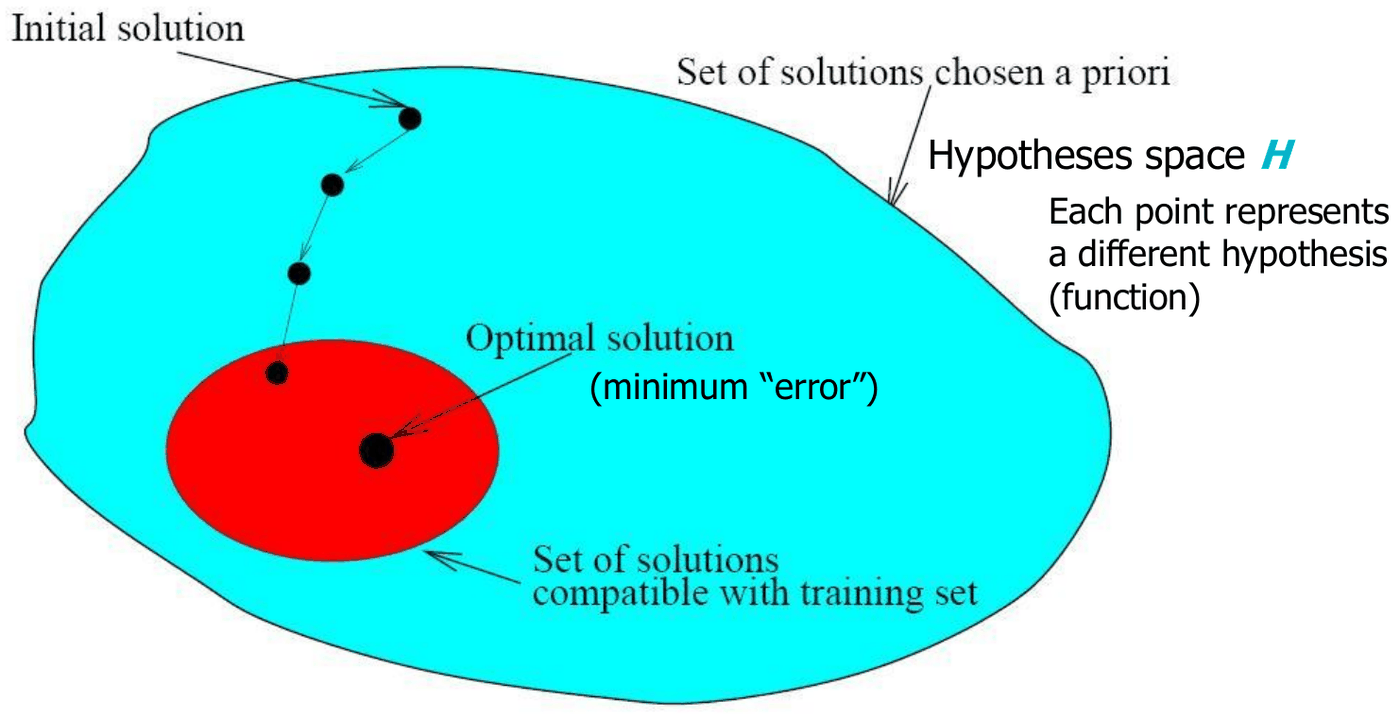
\includegraphics[width=0.77\linewidth,height=0.42\textheight,keepaspectratio]{images/03-l23_ricerca-ipotesi.png}
\caption{Learning as search in the hypothesis space: each point is a
different function; one starts from an initial solution and moves,
typically with local search, towards the minimum-error one.}
\end{figure}

\(H\) may not coincide with the set of all possible functions and the
search cannot be exhaustive: \textbf{assumptions} are needed, and this
is where \textbf{inductive bias} comes into play.

Depending on the context, ``learning'' takes different names:
\textbf{inference} (statistics), \textbf{abduction/induction} (logic),
\textbf{adaptation} (biology, systems), \textbf{optimisation}
(mathematics), \textbf{training} (neural networks), \textbf{function
approximation} (mathematics), regression, \emph{curve fitting}.

After these four ingredients, three concepts remain to be discussed:
\textbf{inductive bias}, \textbf{loss} and \textbf{generalisation}.

\section{Inductive bias}\label{il-bias-induttivo}

To build a model and a learning algorithm we must make
\textbf{assumptions} about the nature of the target function. These can
concern:

\begin{itemize}
\tightlist
\item
  \textbf{constraints on the model}, i.e.\ on the hypothesis space
  \(H\) (the set of hypotheses we can express): this is the
  \textbf{language bias};
\item
  \textbf{constraints or preferences in the learning algorithm}, i.e.\
  in the search strategy: this is the \textbf{search bias};
\item
  both.
\end{itemize}

We will see that these assumptions are \textbf{indispensable} for
obtaining a useful model, i.e.\ one capable of generalising. We study
it with examples in discrete hypothesis spaces, learning a
\textbf{concept} (a Boolean function), as in Mitchell ch.\ 2
(e.g.\ \(h_{cat}(\mathbf{x}) = 1\) if the animal \(\mathbf{x}\) is a
cat, \(0\) otherwise).

\subsection{Learning Boolean functions: an ill-posed
problem}\label{imparare-funzioni-booleane-un-problema-mal-posto}

Suppose we want to learn an unknown Boolean function
\(y = f(x_1, x_2, x_3, x_4)\) from 7 examples.

\begin{figure}[htbp]
\centering
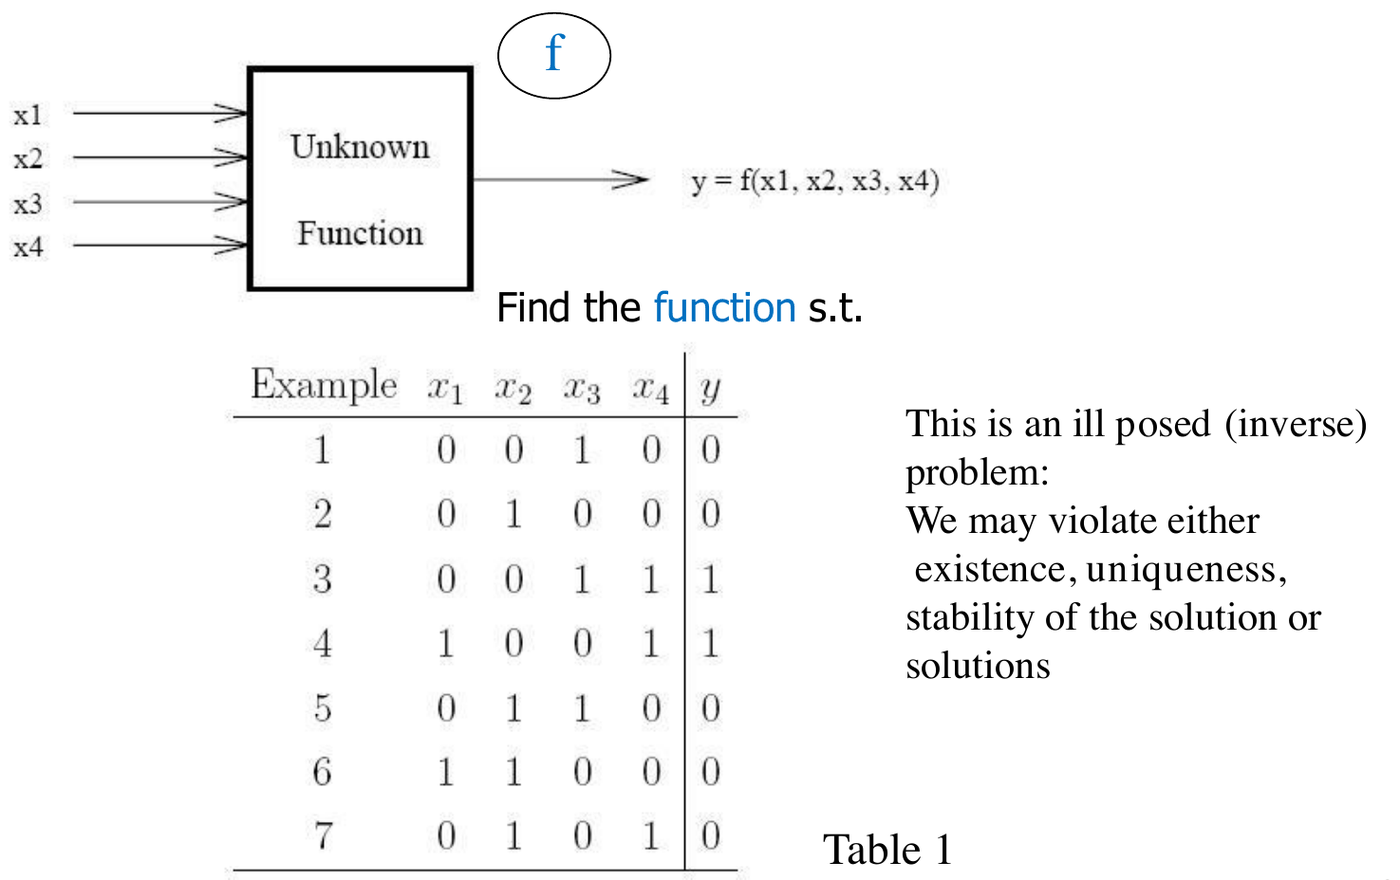
\includegraphics[width=0.77\linewidth,height=0.42\textheight,keepaspectratio]{images/03-l23_funzioni-booleane.png}
\caption{Learning a Boolean function of four variables from seven
examples.}
\end{figure}

This is an \textbf{ill-posed (inverse) problem}: the solution may
violate existence, uniqueness or stability. With 4 binary inputs there
are \(2^4 = 16\) possible input instances and hence \(2^{16} = 65536\)
possible Boolean functions. We cannot know which one is correct until
we see \textbf{all} input-output pairs: after 7 examples there are
still \(2^9 = 512\) possibilities (the 9 unseen instances can have any
output).

In general, for binary inputs and outputs with input dimension \(n\):
\[
|H| = 2^{\#\text{input instances}} = 2^{2^n}.
\]

A model that uses this whole space is a \textbf{lookup table}: a
\emph{rote learner} that memorises the examples and classifies
\(\mathbf{x}\) only if it coincides with an already seen example
(otherwise ``no answer''). \textbf{No inductive bias → no
generalisation.}

\subsection{Restricting the space: conjunctive
rules}\label{restringere-lo-spazio-le-regole-congiuntive}

Let us introduce a \textbf{language bias}: we only consider
\textbf{conjunctive rules}, i.e.\ conjunctions (AND) of literals, such
as \(h_1 = l_2\), \(h_2 = l_1 \wedge l_2\), \(h_3 = \text{true}\),
\(h_4 = \neg l_1 \wedge l_2\). For example ``if \(x_2 = 1\) then
\(h(\mathbf{x}) = 1\), otherwise \(0\)''.

The number of semantically distinct hypotheses collapses: for each of
the \(n\) positions we can have \(l_i\), \(\neg l_i\) or ``don't
care'', giving \(3^n\) hypotheses, plus 1 because all conjunctions
containing \(l_i \wedge \neg l_i\) are equivalent to ``false''. With
\(n = 4\) we go from 65536 to \(3^4 + 1 = 82\) hypotheses.

\begin{boxdefinition}{Consistency and Version Space}

A hypothesis \(h\) is \textbf{consistent} with the training set TR if
\(h(\mathbf{x}) = d(\mathbf{x})\) for every example
\(\langle \mathbf{x}, d(\mathbf{x})\rangle \in TR\).

The \textbf{version space} \(VS_{H,TR}\) is the subset of hypotheses of
\(H\) consistent with all training examples.

\end{boxdefinition}

In this reduced space there are efficient algorithms (Mitchell ch.\ 2)
that find the version space without enumerating all hypotheses.

\subsection{The unbiased learner}\label{lunbiased-learner}

The conjunctive assumption, however, is too restrictive: if the target
concept is not in \(H\) it cannot be represented. For example ``if
\(x_1 = 1\) \textbf{or} \(x_2 = 1\) then 1'' is not a conjunction.

The opposite idea is to choose an \(H\) capable of expressing
\textbf{every teachable concept}: the set of all subsets of the input
space \(X\), i.e.\ the power set \(\mathcal{P}(X)\) (disjunctions,
conjunctions, negations). With \(n = 10\) binary inputs,
\(|X| = 2^{10} = 1024\) and
\(|\mathcal{P}(X)| = 2^{1024} \approx 10^{308}\) concepts --- more than
the atoms in the universe. \(H\) surely contains the target concept.
But what happens to generalisation?

\begin{boxtheorem}{A learner without bias cannot generalise}

With an \emph{unbiased learner}, the only instances classified
unambiguously by the version space are the training examples
themselves: once again we obtain a \textbf{lookup table}.

\textbf{Proof.} Let \(x_i\) be an unseen (test) instance and let
\(h \in VS\). Consider \(h'\) identical to \(h\) everywhere except at
\(x_i\), where \(h'(x_i) \ne h(x_i)\). Since \(H\) contains \emph{all}
functions, \(h' \in H\); and since \(h\) and \(h'\) agree on the
training set, also \(h' \in VS\). Therefore for every hypothesis in the
VS that classifies \(x_i\) as positive there is another that classifies
it as negative: every unseen instance is classified 1 by exactly half
of the hypotheses in the VS and 0 by the other half. The VS cannot give
any answer.

\end{boxtheorem}

\begin{boxexample}{Trivial example}

A single binary input \(x\), \(H = \{x, \neg x, 0, 1\}\) (all possible
functions). The TR contains only \(x = 0 \mapsto d = 0\). The version
space is \(\{x, 0\}\): both are 0 at \(x = 0\). For the test \(x = 1\),
however, \(x\) answers 1 and \(0\) answers 0. There is no way to
decide, unless the whole \(X\) is used as the training set.

\end{boxexample}

\begin{boxtip}{Futility of bias-free learning}

A learner that makes \textbf{no a priori assumptions} about the
identity of the target concept \textbf{has no rational basis} for
classifying unseen instances. Bias (restriction or preference) is not
only useful for efficiency: it is \textbf{necessary for
generalisation}. To learn without bias one would have to show every
single instance of \(X\) as an example. Bias, however, does not yet
tell us \emph{which} solution generalises best.

\end{boxtip}

\subsection{Equivalent inductive and deductive
systems}\label{sistemi-induttivi-e-deduttivi-equivalenti}

An elegant way to see the role of bias: an inductive system (a learning
algorithm that, using the hypothesis space \(H\), receives examples and
a new instance and outputs a classification or ``don't know'') is
\textbf{equivalent to a deductive system} --- a theorem prover --- that
receives the same examples and the same instance \textbf{plus the
inductive bias as an additional axiom}. The inductive bias is therefore
exactly the set of assumptions that makes the classification produced
by the learner ``logically deducible''.

\begin{figure}[htbp]
\centering
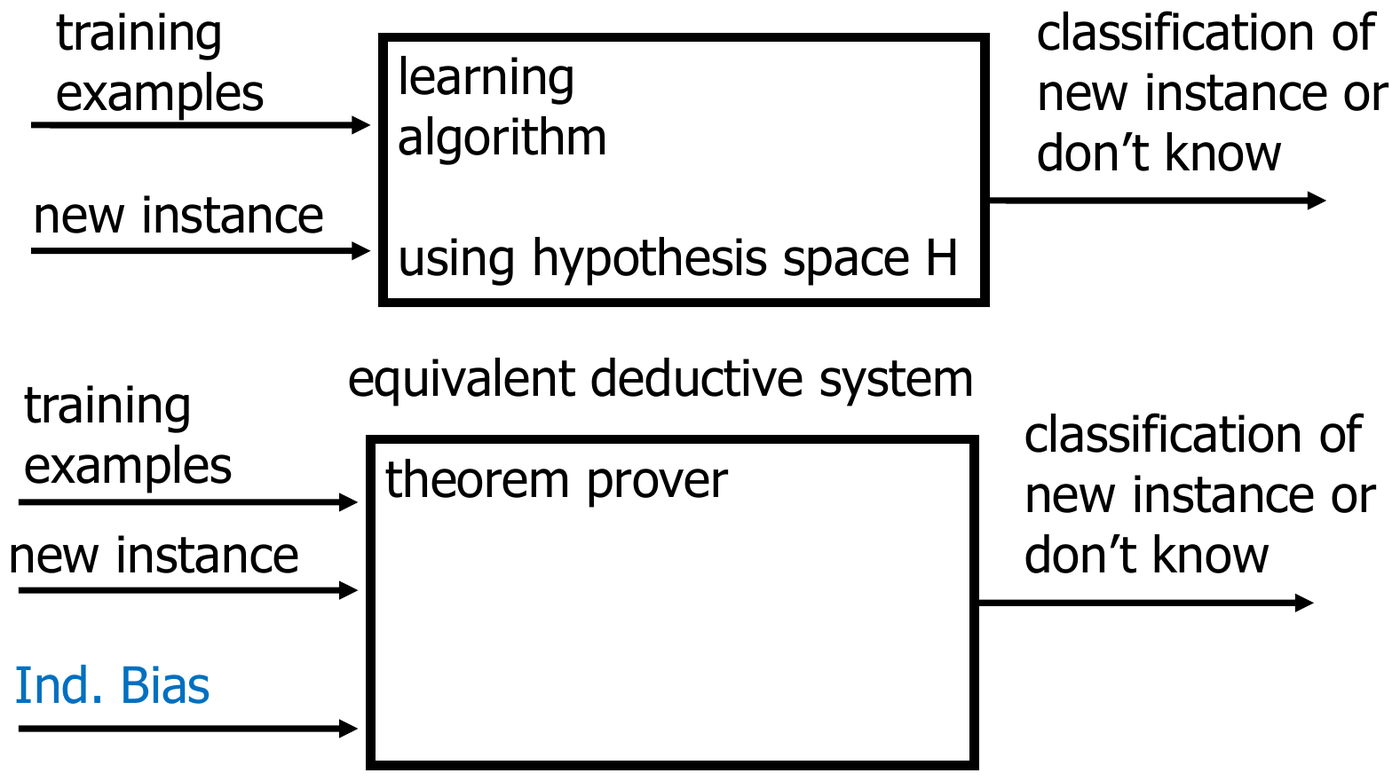
\includegraphics[width=0.80\linewidth,height=0.42\textheight,keepaspectratio]{images/03-l23_sistemi-induttivi.png}
\caption{Inductive bias makes an inductive system equivalent to a
deductive system.}
\end{figure}

\subsection{Language bias or search
bias?}\label{language-bias-o-search-bias}

In modern ML, \textbf{search bias} is generally preferred. Flexible
approaches are used, with very expressive hypothesis spaces and
universal approximation capabilities (neural networks, decision trees),
avoiding language bias and thus \textbf{without excluding a priori} the
target function. Inductive bias remains, but it is entrusted to the
\textbf{search strategy} of the learning algorithm, in practice by
using an \textbf{incomplete} search (which favours certain solutions
over others).

\begin{boxabstract}{Conclusions on inductive bias}

\begin{itemize}
\tightlist
\item
  Learning without bias does not allow extracting regularities from
  data: we get a lookup table, without generalisation.
\item
  \textbf{Every state-of-the-art ML approach has an inductive bias.}
\item
  The problem is characterising the bias of the different models and
  algorithms.
\end{itemize}

\end{boxabstract}

\begin{figure}[htbp]
\centering
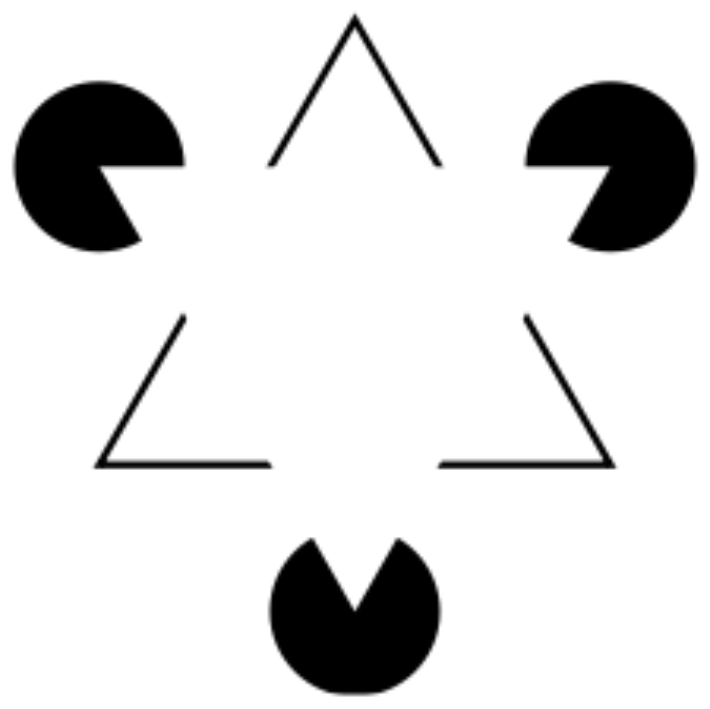
\includegraphics[width=0.37\linewidth,height=0.42\textheight,keepaspectratio]{images/03-l23_kanizsa.png}
\caption{The Kanizsa triangle: an example of perceptual bias of our
visual system, which ``completes'' shapes that are not there.}
\end{figure}

\section{Tasks and loss functions}\label{task-e-funzioni-di-loss}

We said we want to find a ``good'' approximation of \(f\). But how is
the quality of the approximation measured? The model outputs
\(h(\mathbf{x})\) for input \(\mathbf{x}\), and we want to measure the
``distance'' between \(h(\mathbf{x})\) and the target \(d\). An
(``inner'') \textbf{loss function} \(L(h_\mathbf{w}(\mathbf{x}), d)\)
computed on the single pattern is used: a high value indicates a poor
approximation.

\begin{boxdefinition}{Error (Risk, Loss)}

The \textbf{error} is an expected value of the loss \(L\), for example
its mean over the \(l\) samples: \[
\text{Loss}(h_\mathbf{w}) = E(\mathbf{w}) = \frac{1}{l} \sum_{p=1}^{l} L\big(h_\mathbf{w}(\mathbf{x}_p), d_p\big).
\] It serves as the \textbf{objective function} to be minimised during
training and as a measure of error control in the test phase. For now
Error, Risk and Loss are considered synonyms; the differences will be
clarified later.

\end{boxdefinition}

The function \(L\) changes depending on the task. Let us look at the
main cases (useful as a future reference).

\subsection{Regression: squared
error}\label{regressione-errore-quadratico}

\begin{itemize}
\tightlist
\item
  \textbf{Output}: \(d_p = f(\mathbf{x}_p) + e\) (real function plus
  random error).
\item
  \textbf{\(H\)}: a set of real-valued functions.
\item
  \textbf{Loss}: the \textbf{squared error}
  \(L(h_\mathbf{w}(\mathbf{x}_p), d_p) = \big(d_p - h_\mathbf{w}(\mathbf{x}_p)\big)^2\).
\item
  The mean over the dataset is the \textbf{Mean Squared Error} (MSE).
\end{itemize}

\begin{figure}[htbp]
\centering
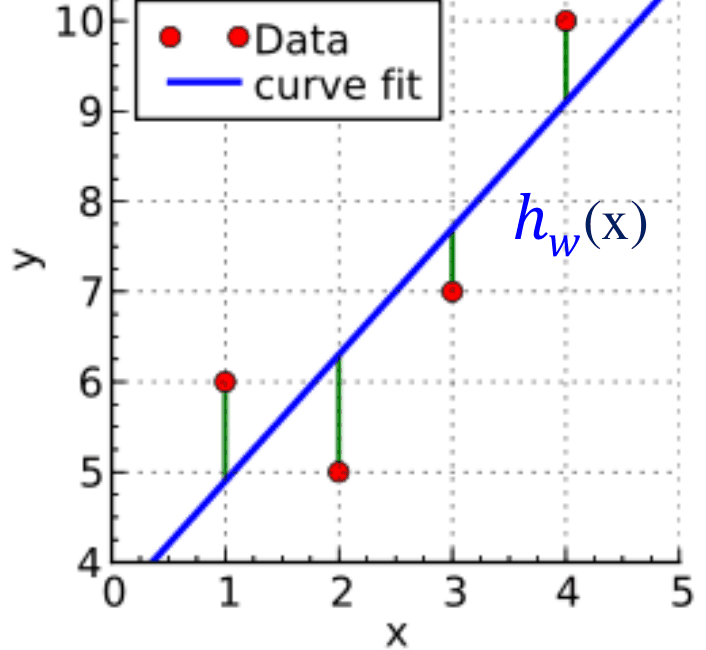
\includegraphics[width=0.43\linewidth,height=0.42\textheight,keepaspectratio]{images/03-l23_mse.png}
\caption{The MSE is the mean of the squares of the green segments,
i.e.\ of the vertical distances between the data (in red) and the line
\(h_w(x) = w_1x + w_0\) (in blue).}
\end{figure}

\[
E(\mathbf{w}) = \frac{1}{l} \sum_{p=1}^{l} \big(y_p - h_\mathbf{w}(\mathbf{x}_p)\big)^2
\] where \(\mathbf{w}\) are the free parameters of the linear model
(in the figure the targets are denoted by \(y\)).

\subsection{Classification: 0/1 loss}\label{classificazione-loss-01}

\begin{itemize}
\tightlist
\item
  \textbf{Output}: for example \(\{0, 1\}\).
\item
  \textbf{\(H\)}: a set of indicator functions.
\item
  \textbf{0/1 loss}: \[
  L(h_\mathbf{w}(\mathbf{x}_p), d_p) = \begin{cases} 0 & \text{if } h_\mathbf{w}(\mathbf{x}_p) = d_p \\ 1 & \text{otherwise} \end{cases}
  \]
\item
  The mean over the dataset is the \textbf{percentage of misclassified
  patterns}: if 20 patterns out of 100 are wrong we have 20\% error,
  i.e.\ 80\% \textbf{accuracy}.
\end{itemize}

\subsection{Clustering and vector quantization
(preview)}\label{clustering-e-vector-quantization-anticipazione}

\begin{itemize}
\tightlist
\item
  \textbf{Goal}: optimally partition an unknown distribution in the
  input space into regions (clusters), each approximated by a
  \textbf{centre} or \textbf{prototype}.
\item
  \textbf{\(H\)}: a set of \emph{vector quantizers}
  \(\mathbf{x} \mapsto c(\mathbf{x})\), which map the continuous space
  into a discrete one.
\item
  \textbf{Loss}: the \textbf{squared distortion}, which measures how
  close the pattern is to the centroid of its cluster: \[
  L(h(\mathbf{x}_p)) = \big(\mathbf{x}_p - h(\mathbf{x}_p)\big) \cdot \big(\mathbf{x}_p - h(\mathbf{x}_p)\big) = \|\mathbf{x}_p - h(\mathbf{x}_p)\|^2.
  \]
\end{itemize}

\subsection{Density estimation
(preview)}\label{stima-di-densituxe0-anticipazione}

\begin{itemize}
\tightlist
\item
  \textbf{Goal}: estimate a density from an assumed class (generative,
  parametric methods).
\item
  \textbf{Output}: a density, for example a normal
  \(p(\mathbf{x} \mid \mu, \sigma^2)\).
\item
  \textbf{\(H\)}: a set of densities (here \(\mu\) and \(\sigma^2\) are
  the two unknown parameters).
\item
  \textbf{Loss}: \(L(h(\mathbf{x}_p)) = -\ln h(\mathbf{x}_p)\), related
  to \textbf{maximising the (log-)likelihood}: minimising the sum of
  \(-\ln\) is equivalent to maximising the product of the probabilities
  of the observed data.
\end{itemize}

\section{Generalisation and
validation}\label{generalizzazione-e-validazione}

This is the \textbf{fundamental concept of the course}.

\begin{itemize}
\tightlist
\item
  \textbf{Learning} is the search for a good function in a function
  space starting from known data, typically by minimising an
  error/loss.
\item
  ``Good'' with respect to the \textbf{generalisation error}: how
  accurately the model predicts on \textbf{new data} (loss measured on
  new data).
\end{itemize}

\begin{boxwarning}{Generalisation is the crucial point}

It is easy to \emph{use} ML tools; it is much harder to use them
\emph{well}. The difference lies entirely in generalisation.

\end{boxwarning}

Two phases are distinguished:

\begin{enumerate}
\def\labelenumi{\arabic{enumi}.}
\tightlist
\item
  \textbf{Learning phase} (\emph{training}, \emph{fitting}): the model
  is built from known data (the training data, plus the bias).
\item
  \textbf{Predictive or test phase} (\emph{deployment}, use of the
  model in inference): the model is applied to new examples. New inputs
  \(\mathbf{x}'\) are taken, the model's response is computed and
  compared with the target \(d'\) that the model has \textbf{never
  seen}: this is how the generalisation capability is evaluated.
\end{enumerate}

\begin{boxnote}{Performance in ML}

In ML, ``performance'' means \textbf{generalisation accuracy} (or
predictive accuracy), estimated by the error computed on a
\textbf{test set} kept aside (\emph{hold out}).

\end{boxnote}

\textbf{Statistical Learning Theory} (Vapnik) studies the mathematical
conditions under which a model is able to generalise; its basics will
be seen in the next lecture.

Evaluating the performance of an ML system coincides with evaluating
its predictive accuracy: in a word, \textbf{validation! validation!
validation!} Validation techniques serve both to \textbf{evaluate}
generalisation (\emph{model assessment}) and to \textbf{manage} it
(\emph{model selection}), and will be the subject of the next lecture.

\begin{boxnote}{The cost of inference}

Even the inference phase alone (the input → output \emph{mapping}) can
be costly when there are millions of requests, as in Google's services:
this is why dedicated chips such as \textbf{Tensor Processing Units}
(TPUs) were designed, originally conceived for TensorFlow.

\end{boxnote}

\begin{boxabstract}{Summary}

ML builds a hypothesis \(h\) that approximates an unknown function
\(f\) from examples. Its ingredients are \textbf{data}
(representation, encoding, noise), \textbf{task} (supervised:
classification and regression; unsupervised: clustering, density),
\textbf{model} (which defines the hypothesis space \(H\)),
\textbf{learning algorithm} (search in \(H\) for the minimum-error
hypothesis) and \textbf{validation}. Without \textbf{inductive bias}
there is no generalisation; in modern ML \emph{search bias} with very
expressive models is preferred. Quality is measured with a
\textbf{loss} that depends on the task (squared, 0/1, distortion,
\(-\ln\)), but what really matters is the error on \textbf{new data}.

\end{boxabstract}

\begin{boxquestion}{Possible exam questions}

\begin{itemize}
\tightlist
\item
  What is inductive bias? What is the difference between language bias
  and search bias?
\item
  Prove that an \emph{unbiased learner} cannot generalise.
\item
  How many hypotheses are there with \(n\) binary inputs without
  constraints? And with conjunctive rules only?
\item
  What is the version space?
\item
  Which losses are used for regression, classification, clustering and
  density estimation?
\item
  What is meant by generalisation and how is it estimated?
\end{itemize}

\end{boxquestion}
